\chapter{Increment three}
\label{chap:Increment three}
The procedure of this increment will be the same as the previous ones. The requirements from section \ref{sec:i2Evaluation} in increment two, will be the base for this increment. The requirements in focus will be discussed, tried implemented and the evaluated upon, which might lead to changes of the requirements list. 

\section{Requirements}
\label{sec:i3Requirements}

\begin{itemize}
	\item The trash bin should catch the trash if the user throws it towards the trash bin and within a predefined area
	\begin{itemize}
		\item {The robots predefined area should be calculated from the hardware limitations of the motors’ speed}
	\end{itemize}
	\item The robot should know where it is positioned
	\begin{itemize}
		\item {The robot should have a starting position, from where it should be able to calculate it's current position through calculations of the motor encoders}
		\item {The robot's starting point should be placed outside its predefined area, such that it moves forward into the area}
	\end{itemize}
	\item The robot should be able to detect and track the thrown trash
	\begin{itemize}
		\item {The thrown trash should be detected and tracked by a Microsoft Kinect}
		\item {The Kinect should send the coordinates of the impact point of the trash to the robot}
	\end{itemize}
	\item The robot should be able to calculate the impact point for the object
	\begin{itemize}
		\item {Trajectory prediction should be used to calculate impact point of the thrown trash}
	\end{itemize}
	\item The robot should be able to move the trash bin, such that the thrown trash lands inside the bin
	\begin{itemize}
		\item {The robot should be able to turn and drive forward}
		\item\textcolor{blue}{The robot should be able to recognize the coordinates sent from the Kinect}
	\end{itemize}
	\item {The robot should be able to receive data from a computer, through a wireless network}
	\item \textcolor{blue}{The system tasks should be able to be scheduled and verified}
\end{itemize}

\section{System design}
\label{sec:i3System design}
This section will describe and explain the marked requirements, for how they are planned to be fulfilled.

\subsection{Connecting Arduino and Kinect}
\label{sec:i3Connecting Arduino and Kinect system design}
For connecting the Arduino and Kinect, the Wifi library is used as explained in Appendix \ref{sec:Connecting Arduino and Kinect}. The Kinect should create a TCP-client, which should send the appropriate data to the Arduino. This TCP-client should connect when it can send data, and disconnect after sending the data, since the Arduino has a timer that closes the connection after 10 seconds of inactivity. The sent data should be of the form (x, z) expressing the distance from the kinect to the impact point of the object and the ground. The x-coordinate should express the horizontal position, and the z-coodinate should express the depth position. As the Kinect camera should be position and tilted so that the bottom angle of the cameras point of view is parallel to the ground, makes the y coordinate useless, as the impact point would always be at (x, (y = 0), z). This delimitation also gives the camera a sense of where the ground is, since it would not be able to see the ground, and therefore would calculate a different impact point, as the object would in a sense fall through the ground in the picture. 

\subsection{Scheduling}
\label{sec:i3Scheduling}
The calculation for the WCET of the system is described in chapter \ref{chap:Implementation} section \ref{sec:Scheduling implementation}.

The WCET for the two functions and the time spent on sending data from the Kinect via wifi ,using the Micros() function, is listed below:
\begin{itemize}
	\item updatePosAndHead = 1076 microseconds
	\item driveTowardsGoal = 732 microseconds
	\item WiFi = 8433 microseconds
\end{itemize}

The above results will be used for a schedulability analysis made in UPPAAL in section \ref{sec:i3UPPAAL model}. 
\section{Implementation}
\label{sec:i3Implementation}
This section will describe if the requirements were fulfilled through implementation.

\subsection{Connecting Arduino and Kinect}
\label{sec:i3Connecting Arduino and Kinect implementation}

When the Kinect sensor has spotted the object in several frames, it returns a function that gives the objects position in relation to a given time in the future.
The position given is in three dimensions, but only the x and y-coordinate are of interest, because the coordinate is only returned when we know the object must have hit the ground. The x-coordinate is given in meters, in relation to the Kinects left field of view. The y-coordinate is also given in meters, and is the distance between the balls impact spot with the ground, and the Kinect itself. This can be seen in \ref{FieldOfView}

\begin{figure}[h]
	\centering
	\fbox{\includegraphics[scale=0.35]{billeder/FieldOfView11.png}}
	\caption{Object impact in relation to Kinect}
	\label{FieldOfView}
\end{figure}

This information is not useful to the Arduino as is, so the coordinate must be converted to a coordinate that is more useful to the Arduino.
Looking at \ref{FieldOfView}, the length xdist represents the distance from the Kinects field of view to the impact point of the object, and the zdist represents the distance between the Kinect and the impact point of the object. This is the information given by the Kinect library.
Since this coordinate system is not straight in relation to the Kinect and changes from impact to impact, depending on the depth, we first calculate the impact point as shown by a and b on \ref{FieldOfView2}.

\begin{figure}[h]
	\centering
	\fbox{\includegraphics[scale=0.35]{billeder/FieldOfView3.png}}
	\caption{Object impact in relation to Kinect with calculated a and b, and the Arduino}
	\label{FieldOfView2}
\end{figure}

The code for calculating the coordinates using trigonometry, where XSquare is a and YSquare is b on figure:

\begin{lstlisting}[caption={Converting coordinates form Kinect}, label={convertCoordinate}]
double as1 = (Math.Sin(2.06821516));
double as2 = as1 * Math.Abs(Xdist);
double as3 = (ZDist);
double as4 = as2 / as3;
double A = Math.Asin(as4);
A = A * 180 / Math.PI;
double B = 180 - A - 118.5;
double b = ((Math.Sin(B * Math.PI / 180)) * Math.Abs(v3.X)) / (Math.Sin(A * Math.PI / 180));
double A2 = 90 - B;
double XSquare = ((Math.Sin(A2 * Math.PI / 180)) * (v3.Z - 0.5)) / (Math.Sin(90 * Math.PI / 180));
double YSquare = ((Math.Sin(B * Math.PI / 180)) * (v3.Z - 0.5)) / (Math.Sin(90 * Math.PI / 180));
\end{lstlisting}

Using the calculated a and b, it is only a matter of addition and subtraction, to match the Arduinos coordinate system, based on its distance from the Kinect.

The coordinate is the send to the Arduino, using a TCP connection.
The code for this is shown here:
\begin{lstlisting}[caption={Sending data to the Arduino}, label={sendData}]
tcpClient = new TcpClient();
tcpClient.Connect("192.168.0.100", 9999);
stream = tcpClient.GetStream();

stream.Write(Encoding.UTF8.GetBytes((finalx.ToString() + ";" + finaly.ToString()).ToCharArray()), 0, (finalx.ToString() + ";" + finaly.ToString()).Length);
tcpClient.Close();
\end{lstlisting}

A new TCP connection is opened by using the Arduinos IP-address, which is then used, by writing to its stream.
When this code has executed, the Arduino has the information ready.

\subsection{UPPAAL model of schedulability}
\label{sec:i3UPPAAL model}
To create the UPPAAL model and to check the schedulability of the tasks used for Dumpsty, every tasks WCET is calculated. This execution time is attained through running the code multiple times with a set timer, and writing the timer in a log after executing the specific task. There are four tasks for Dumpsty: Updating the position and heading (referred to as "PrA"), driving towards the goal position ("PrB"), the WiFi code that has to be looped ("PrC") and the delay to not execute the tasks seven times within the deadline ("PrD"). Here are the WCET attained through the tests, and to the right of the clock cycles is the WCET used in UPPAAL. The WCET used in UPPAAL has a significant margin greater than the WCET gained through the tests, since there is enough time to give each task a greater WCET, and the worst case tested is not necessarily the WCET of the tasks. 

\begin{itemize}
	\item PrA \tab Tested: 1067 microseconds \tab UPPAAL: 2 milliseconds
	\item PrB \tab Tested: 732  microseconds \tab UPPAAL: 1 milliseconds
	\item PrC \tab Tested: 8469 microseconds \tab UPPAAL: 9 milliseconds
	\item PrD \tab Tested: 10000 microseconds \tab UPPAAL: 10 milliseconds
\end{itemize}

The interrupt generated by the motor encoders is taken into account in every task, but to simplify the schedulability analysis, the WCET of the interrupt has been multiplied to the WCET of every greater task. Therefore the interrupt and the interrupt handler is not considered as a task, but as a part of the other tasks.

When describing these tasks in UPPAAL, two different classes were declared: One to instantiate a cyclic executive task instance of every task, and a CPU class to control the synchronization between all the tasks, as shown in the following figure:

\begin{figure}[h]
	\centering
	\fbox{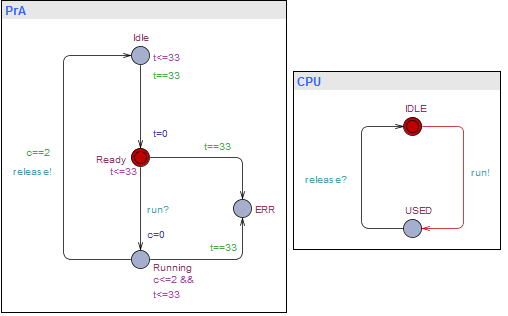
\includegraphics[scale=0.60]{billeder/UPPAALPr}}
	\caption{Automata in UPPAAL}
	\label{UppaalModelAutomata}
\end{figure}

When the automata of the tasks has been created, every task has to be declared with an ID, a deadline and a period. The deadline has been declared for every task to be within the MIT of coordinates from the Kinect sensor, which is 33 milliseconds.
The tasks are declared as:

\begin{itemize}
	\item PrA = TASK(1, 33, 2);
	\item PrB = TASK(2, 33, 1);
	\item PrC = TASK(3, 33, 9);
	\item PrD = TASK(4, 33, 10);
\end{itemize}

After creating the automata and declaring the tasks, the UPPAAL schedulability analysis can be done. This is done through the verifier in UPPAAL, with two different queries:

\begin{lstlisting}[caption={Queries for UPPAAL}, label={QueriesAppendix}]
	E<> PrA.Ready and PrB.Ready and PrC.Ready and PrA.t==0 and PrB.t==0 and PrC.t==0 and time>0
	E[] not (PrA.ERR or PrB.ERR or PrC.ERR)
\end{lstlisting}

The first query dictates that each tasks instance should be in a ready state, each tasks should have completed within the deadline and some interval of time has to be passed. This creates a scenario where the tasks has all been executed, and none of them have exceeded the deadline.
The second query dictates that no task should ever enter an error state.
After verifying both queries it is possible to say whether the tasks can be scheduled or not, in this case it is possible.

\section{Evaluation}
\label{sec:i3Evaluation}
Many different methods were used to try to calculate the WCET for the systems functions. At first it was tried to count the clock cycles from the complied assembly code, which proved to be very difficult, since the bounds of the libraries was unknown. Because of these problems third party software and libraries was used to calculate the WCET, but the once again without any success. The method used to calculate the WCET was to use the micros() function, available in the arduino IDE, to measure the time used on the function, which would give close to a WCET of the functions. The tasks all had a significant margin to improve the possibility of hitting actual WCET. \newline
The WCET's were used with the software UPPALL, as described in section \ref{sec:i3UPPAAL model}. This concluded that the tasks was easily schedulable within the defined deadlines.

%EVALUERE PÅ CONNECTING ARDUINO AND KINECT!!!!!!!!!!!!!!

After finalizing increment three the requirements in the following list will be the final requirements for the system:

\begin{itemize}
	\item The trash bin should catch the trash if the user throws it towards the trash bin and within a predefined area
	\begin{itemize}
		\item {The robots predefined area should be calculated from the hardware limitations of the motors’ speed}
	\end{itemize}
	\item The robot should know where it is positioned
	\begin{itemize}
		\item {The robot should have a starting position, from where it should be able to calculate it's current position through calculations of the motor encoders}
		\item {The robot's starting point should be placed outside its predefined area, such that it moves forward into the area}
	\end{itemize}
	\item The robot should be able to detect and track the thrown trash
	\begin{itemize}
		\item {The thrown trash should be detected and tracked by a Microsoft Kinect}
		\item {The Kinect should send the coordinates of the impact point of the trash to the robot}
	\end{itemize}
	\item The robot should be able to calculate the impact point for the object
	\begin{itemize}
		\item {Trajectory prediction should be used to calculate impact point of the thrown trash}
	\end{itemize}
	\item The robot should be able to move the trash bin, such that the thrown trash lands inside the bin
	\begin{itemize}
		\item {The robot should be able to turn and drive forward}
		\item\textcolor{green}{The robot should be able to recognize the coordinates sent from the Kinect}
	\end{itemize}
	\item {The robot should be able to receive data from a computer, through a wireless network}
	\item \textcolor{green}{The system tasks should be able to be scheduled and verified}
\end{itemize}
